\documentclass{standalone}

\usepackage{tikz}
\usetikzlibrary{calc}

\begin{document}
  %noformat{
  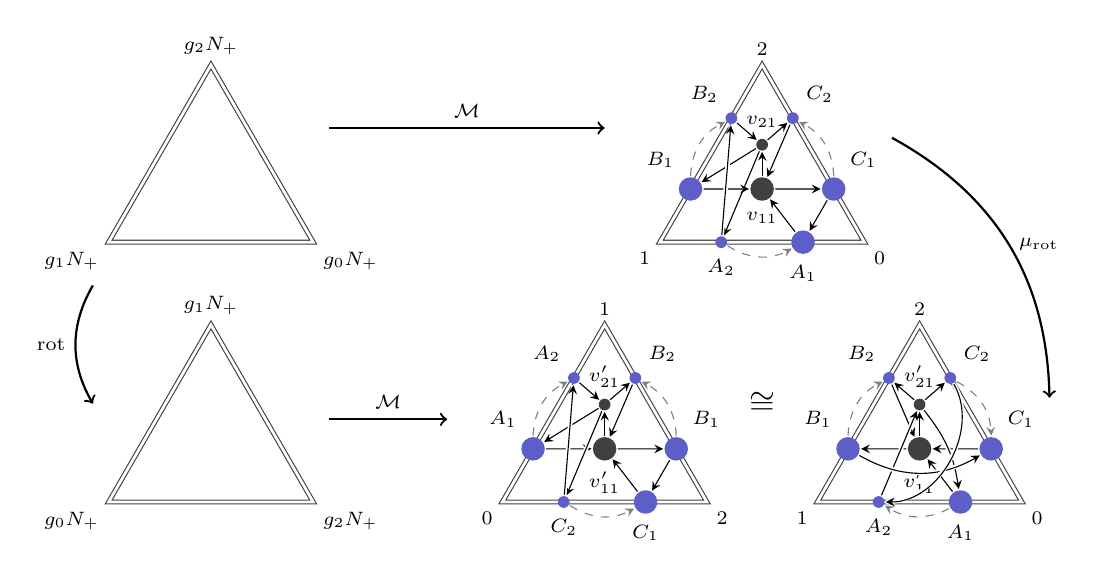
\begin{tikzpicture}
    \tikzstyle{v1} = [circle, outer sep=0.5pt, fill, inner sep=1.5pt]
    \tikzstyle{v2} = [circle, outer sep=0.5pt, fill, inner sep=3.0pt]
    \tikzstyle{unf} = [color=darkgray]
    \tikzstyle{frz} = [color=blue!60!darkgray!70]
    \tikzstyle{r} = [color=red!70!darkgray!70]
    \tikzstyle{e} = [->, >={stealth}, preaction={draw=white, -, ultra thick}]
    \tikzstyle{b} = [fill, fill opacity=0.0, circle, outer sep=0.5pt, inner sep=1.5pt]
    \tikzstyle{te} = [color=darkgray, double distance=1pt]
    \tikzstyle{h} = [dashed, color=gray, ->, >={stealth}]

    \tikzset{font=\scriptsize}

    \begin{scope}[shift={(0,3.3)}]
      \coordinate[label={210:$g_1 N_{+}$}] (l_0) at (210:1.5);
      \coordinate[label={ 90:$g_2 N_{+}$}] (l_1) at ( 90:1.5);
      \coordinate[label={330:$g_0 N_{+}$}] (l_2) at (-30:1.5);

      \draw[te] (l_0) -- (l_1) -- (l_2) -- cycle;
    \end{scope}

    \begin{scope}[shift={(0,0)}]
      \coordinate[label={210:$g_0 N_{+}$}] (l_0) at (210:1.5);
      \coordinate[label={ 90:$g_1 N_{+}$}] (l_1) at ( 90:1.5);
      \coordinate[label={330:$g_2 N_{+}$}] (l_2) at (-30:1.5);

      \draw[te] (l_0) -- (l_1) -- (l_2) -- cycle;
    \end{scope}

    \begin{scope}[shift={(7,3.3)}]
      \coordinate[label={330:$0$}] (l_0) at (-30:1.5);
      \coordinate[label={210:$1$}] (l_1) at (210:1.5);
      \coordinate[label={ 90:$2$}] (l_2) at ( 90:1.5);

      \draw[te] (l_0) -- (l_1) -- (l_2) -- cycle;

      \node[v2, frz, label={120:$B_1$}   ] (B1)  at ($ (l_1)!0.3!(l_2) $) {};
      \node[v1, frz, label={120:$B_2$}   ] (B2)  at ($ (l_1)!0.7!(l_2) $) {};
      \node[v1, frz, label={270:$A_2$}   ] (A2)  at ($ (l_1)!0.3!(l_0) $) {};
      \node[v2, frz, label={270:$A_1$}   ] (A1)  at ($ (l_1)!0.7!(l_0) $) {};
      \node[v2, frz, label={ 60:$C_1$}   ] (C1)  at ($ (l_2)!0.7!(l_0) $) {};
      \node[v1, frz, label={ 60:$C_2$}   ] (C2)  at ($ (l_2)!0.3!(l_0) $) {};
      \coordinate (e01mid) at ($ (l_0)!0.5!(l_1) $);
      \node[v2, unf, label={270:$v_{11}$}] (v11) at ($ (l_2)!0.70!(e01mid) $) {};
      \node[v1, unf, label={ 90:$v_{21}$}] (v21) at ($ (l_2)!0.45!(e01mid) $) {};

      \draw[h] (A2) to[bend right] (A1);
      \draw[h] (B1) to[bend left] (B2);
      \draw[h] (C1) to[bend right] (C2);

      \draw[e] (v11) -- (v21);
      \draw[e] (v11) -- ( C1);
      \draw[e] (v21) -- ( B1);
      \draw[e] (v21) -- ( C2);
      \draw[e] (v21) -- ( A2);
      \draw[e] ( B1) -- (v11);
      \draw[e] ( B2) -- (v21);
      \draw[e] ( C1) -- ( A1);
      \draw[e] ( C2) -- (v11);
      \draw[e] ( A1) -- (v11);
      \draw[e] ( A2) -- ( B2);
    \end{scope}

    \begin{scope}[shift={(9,0)}]
      \coordinate[label={210:$1$}] (l_1) at (210:1.5);
      \coordinate[label={ 90:$2$}] (l_2) at ( 90:1.5);
      \coordinate[label={330:$0$}] (l_0) at (-30:1.5);

      \draw[te] (l_0) -- (l_1) -- (l_2) -- cycle;

      \node[v2, frz, label={120:$B_1$}   ] (B1)  at ($ (l_1)!0.3!(l_2) $) {};
      \node[v1, frz, label={120:$B_2$}   ] (B2)  at ($ (l_1)!0.7!(l_2) $) {};
      \node[v1, frz, label={270:$A_2$}   ] (A2)  at ($ (l_1)!0.3!(l_0) $) {};
      \node[v2, frz, label={270:$A_1$}   ] (A1)  at ($ (l_1)!0.7!(l_0) $) {};
      \node[v2, frz, label={ 60:$C_1$}   ] (C1)  at ($ (l_2)!0.7!(l_0) $) {};
      \node[v1, frz, label={ 60:$C_2$}   ] (C2)  at ($ (l_2)!0.3!(l_0) $) {};
      \coordinate (e01mid) at ($ (l_0)!0.5!(l_1) $);
      \node[v2, unf, label={269:$v_{11}'$}] (v11) at ($ (l_2)!0.70!(e01mid) $) {};
      \node[v1, unf, label={ 90:$v_{21}'$}] (v21) at ($ (l_2)!0.45!(e01mid) $) {};

      \draw[h] (A1) to[bend left ] (A2);
      \draw[h] (B1) to[bend left ] (B2);
      \draw[h] (C2) to[bend left ] (C1);

      \draw[e] (v11) -- (v21);
      \draw[e] ( C1) -- (v11);
      \draw[e] ( A1) -- (v11);
      \draw[e] (v11) -- ( B1);
      \draw[e] ( B2) -- (v11);
      \draw[e] (v21) -- ( C2);
      \draw[e] (v21) -- ( B2);
      \draw[e] ( A2) -- (v21);
      \draw[e] (v21) to[bend left=15 ] ( A1);
      \draw[e] ( B1) to[bend right   ] ( C1);
      \draw[e] ( C2) to[bend left=60 ] ( A2);
    \end{scope}

    \begin{scope}[shift={(5,0)}]
      \coordinate[label={210:$0$}] (l_0) at (210:1.5);
      \coordinate[label={ 90:$1$}] (l_1) at ( 90:1.5);
      \coordinate[label={330:$2$}] (l_2) at (-30:1.5);

      \draw[te] (l_0) -- (l_1) -- (l_2) -- cycle;

      \node[v2, frz, label={ 60:$B_1$}   ] (B1)  at ($ (l_1)!0.7!(l_2) $) {};
      \node[v1, frz, label={ 60:$B_2$}   ] (B2)  at ($ (l_1)!0.3!(l_2) $) {};
      \node[v1, frz, label={120:$A_2$}   ] (A2)  at ($ (l_1)!0.3!(l_0) $) {};
      \node[v2, frz, label={120:$A_1$}   ] (A1)  at ($ (l_1)!0.7!(l_0) $) {};
      \node[v2, frz, label={270:$C_1$}   ] (C1)  at ($ (l_0)!0.7!(l_2) $) {};
      \node[v1, frz, label={270:$C_2$}   ] (C2)  at ($ (l_0)!0.3!(l_2) $) {};
      \coordinate (e02mid) at ($ (l_0)!0.5!(l_2) $);
      \node[v2, unf, label={270:$v_{11}'$}] (v11) at ($ (l_1)!0.70!(e02mid) $) {};
      \node[v1, unf, label={ 90:$v_{21}'$}] (v21) at ($ (l_1)!0.45!(e02mid) $) {};

      \draw[h] (A1) to[bend left ] (A2);
      \draw[h] (B1) to[bend right] (B2);
      \draw[h] (C2) to[bend right] (C1);

      \draw[e] (v11) -- (v21);
      \draw[e] ( C1) -- (v11);
      \draw[e] ( A1) -- (v11);
      \draw[e] (v11) -- ( B1);
      \draw[e] ( B2) -- (v11);
      \draw[e] (v21) -- ( C2);
      \draw[e] (v21) -- ( B2);
      \draw[e] ( A2) -- (v21);
      \draw[e] (v21) -- ( A1);
      \draw[e] ( B1) -- ( C1);
      \draw[e] ( C2) -- ( A2);
    \end{scope}

    \draw[->, thick] ( 1.5, 0.3) to node[midway, above] (t01) {$\mathcal{M}$} ( 3.0, 0.3);
    \draw[->, thick] ( 1.5, 4.0) to node[midway, above] (t02) {$\mathcal{M}$} ( 5.0, 4.0);
    \draw[->, thick] (-1.5, 2.0) to[bend right] node[midway, left] (t03) {rot} (-1.5, 0.5);
    \draw[->, thick]
        ($ (7,3.5) + (90:1.5)!0.5!(-30:1.5) + (0:1) $)
        to[bend left] node[midway, right] (t04) {$\mu_{\mathrm{rot}}$}
        ($ (9,0.2) + (90:1.5)!0.5!(-30:1.5) + (0:1) $);
    \node (t05) at ( 7.0, 0.5) {\large $\cong$};
  \end{tikzpicture}
  %}noformat
\end{document}
